\documentclass[12pt, letterpaper]{article}
\usepackage[margin=1in]{geometry}
\usepackage[T1]{fontenc}
\usepackage{lmodern}
\usepackage{cmap}
\usepackage[utf8]{inputenc}
\usepackage{amsmath, amssymb, amsthm}
\usepackage{mathtools}
\usepackage{enumitem}
\usepackage{booktabs}
\usepackage{xcolor}
\usepackage{titlesec}
\usepackage{parskip}
\usepackage{hyperref}
\usepackage{fancyhdr}
\usepackage{tcolorbox}
\usepackage{graphicx}
\usepackage{caption}
\tcbuselibrary{skins, breakable}

\definecolor{darkblue}{RGB}{15,55,115}
\definecolor{midblue}{RGB}{30,100,180}
\definecolor{theorybg}{RGB}{245,250,255}
\definecolor{questionbg}{RGB}{255,252,240}
\definecolor{evencolor}{RGB}{60,0,100}

\hypersetup{colorlinks=true,linkcolor=darkblue,urlcolor=midblue,
  pdftitle={Ljungqvist \& Sargent --- Recursive Macroeconomic Theory --- Complete Solutions, Chapter 3}}

\setlength{\headheight}{14pt}
\pagestyle{fancy}
\fancyhf{}
\renewcommand{\headrulewidth}{0.4pt}
\fancyhead[L]{\small\textcolor{darkblue}{\textit{Ljungqvist \& Sargent --- Recursive Macroeconomic Theory}}}
\fancyhead[R]{\small\textcolor{darkblue}{\thepage}}
\fancyfoot[C]{\small\textcolor{gray}{Complete Solutions --- Chapter 3}}

\titleformat{\section}[block]
  {\large\bfseries\color{darkblue}}{}{0pt}{}
  [\vspace{2pt}\color{darkblue}\rule{\textwidth}{1.5pt}\vspace{4pt}]

\titleformat{\subsection}[block]
  {\normalsize\bfseries\color{midblue}}{}{0pt}{}
  [\vspace{1pt}\color{midblue}\rule{0.5\textwidth}{0.8pt}\vspace{3pt}]

\tcbset{
  theorybox/.style={
    enhanced,breakable,colback=theorybg,colframe=darkblue,
    fonttitle=\bfseries\small\color{darkblue},boxrule=0.5pt,arc=3pt,
    left=6pt,right=6pt,top=4pt,bottom=4pt,title={Key Theory},
  },
  questionbox/.style={
    enhanced,breakable,colback=questionbg,colframe=gray!60,
    fonttitle=\bfseries\small\color{gray!60!black},boxrule=0.4pt,arc=2pt,
    left=6pt,right=6pt,top=4pt,bottom=4pt,title={\textit{Question}},
  },
  oddbox/.style={
    enhanced,breakable,colback=white,colframe=darkblue,
    attach boxed title to top left={yshift=-2mm,xshift=6mm},
    boxed title style={colback=darkblue,colframe=darkblue,arc=2pt,
      boxrule=0pt,left=6pt,right=6pt,top=3pt,bottom=3pt},
    fonttitle=\bfseries\large\color{white},
    boxrule=0.8pt,arc=3pt,
    left=8pt,right=8pt,top=10pt,bottom=6pt,
  },
  evenbox/.style={
    enhanced,breakable,colback=white,colframe=evencolor,
    attach boxed title to top left={yshift=-2mm,xshift=6mm},
    boxed title style={colback=evencolor,colframe=evencolor,arc=2pt,
      boxrule=0pt,left=6pt,right=6pt,top=3pt,bottom=3pt},
    fonttitle=\bfseries\large\color{white},
    boxrule=0.8pt,arc=3pt,
    left=8pt,right=8pt,top=10pt,bottom=6pt,
  },
  databox/.style={
    enhanced,breakable,colback=gray!8,colframe=gray!55,
    fonttitle=\bfseries\small\color{gray!60!black},boxrule=0.4pt,arc=2pt,
    left=6pt,right=6pt,top=4pt,bottom=4pt,title={Numerical exercise --- see the companion code},
  },
  trapbox/.style={
    enhanced,breakable,colback=red!4,colframe=red!45!black,
    fonttitle=\bfseries\small\color{white},boxrule=0.4pt,arc=2pt,
    coltitle=white,
    left=6pt,right=6pt,top=4pt,bottom=4pt,title={Where this goes wrong},
  },
}

\newcommand{\pd}[2]{\dfrac{\partial #1}{\partial #2}}
\newcommand{\dd}[2]{\dfrac{d #1}{d #2}}
\newcommand{\MRS}{\mathrm{MRS}}
\newcommand{\MRT}{\mathrm{MRT}}
\newcommand{\MU}{\mathrm{MU}}
\newcommand{\Var}{\mathrm{Var}}
\newcommand{\Cov}{\mathrm{Cov}}
\newcommand{\E}{\mathrm{E}}
\newcommand{\MPK}{\mathrm{MPK}}
\newcommand{\MPL}{\mathrm{MPL}}
\newcommand{\stst}{^{\ast}}

\setlist[enumerate,1]{label=(\alph*),itemsep=6pt,parsep=2pt}
\setlist[enumerate,2]{label=(\roman*),itemsep=3pt}

\begin{document}

%======================================================================
% TITLE PAGE
%======================================================================
\begin{titlepage}
\centering
\vspace*{2.5cm}
{\Huge\bfseries\color{darkblue} Recursive Macroeconomic Theory\par}
\vspace{6pt}
{\large Lars Ljungqvist \& Thomas J. Sargent (4th ed., 2018)\par}
\vspace{1.4cm}
{\LARGE\bfseries Complete Solutions\par}
\vspace{6pt}
{\LARGE\bfseries Chapter 3 --- Dynamic Programming\par}
\vspace{1.2cm}
{\large The single end-of-chapter exercise, 3.1 (p.~114)\par}
\vspace{2cm}

\begin{tcolorbox}[theorybox,title={What is in this file},width=0.86\textwidth]
\small
Chapter 3 closes with one exercise, \emph{Howard's policy iteration algorithm} on the
stochastic Brock--Mirman model. It is analytical: it asks to show that the algorithm lands on
the optimal policy in a single step. The solution below does every step of the algebra, and
derives the closed form of the value of an arbitrary policy by two independent routes.

\smallskip
The companion notebook \texttt{ls\_ch03.ipynb} (same folder) checks each analytical claim
numerically --- series, recursion and Monte Carlo for the policy value; a numerical
maximisation with Gauss--Hermite quadrature for the improvement step; the Bellman residual ---
and then solves a discretised version by value iteration and policy iteration. Every check is
an \texttt{assert}.

\smallskip
Notation follows the book: $k$ capital, $\theta$ the productivity shock, $h$ a policy,
$J_h$ the value of following it forever. Blue boxes are odd-numbered exercises.
\end{tcolorbox}

\vfill
{\small MPE Insper --- Macroeconomia I --- 2026, 3\textordmasculine{} trimestre\par}
\end{titlepage}

\tableofcontents
\newpage

%======================================================================
\section{Chapter 3 \quad Dynamic Programming}
%======================================================================

\begin{tcolorbox}[theorybox,title={Chapter 3 Overview}]
The chapter replaces the search for an infinite \emph{sequence} of controls by the search
for a pair of \emph{functions}: a value function $V(x)$ and a policy $u=h(x)$ linked by the
Bellman equation (3.1.5),
\[
V(x)=\max_u\{r(x,u)+\beta V[g(x,u)]\}.
\]
\textbf{Three methods} (section 3.1.1) solve it:
\begin{itemize}[itemsep=1pt]
\item \emph{Value function iteration} (3.1.10): $V_{j+1}(x)=\max_u\{r(x,u)+\beta V_j(\tilde x)\}$
from $V_0=0$. Converges at a linear (geometric) rate.
\item \emph{Guess and verify}: posit a functional form with undetermined coefficients, as in
(3.1.12)--(3.1.14).
\item \emph{Howard's improvement algorithm}: (1) evaluate a policy,
$V_{h_j}(x)=\sum_t\beta^t r[x_t,h_j(x_t)]$; (2) improve it,
$h_{j+1}=\arg\max_u\{r(x,u)+\beta V_{h_j}[g(x,u)]\}$; (3) repeat. It is Newton's method on the
Bellman equation (footnote 6), so it converges quadratically.
\end{itemize}
\textbf{The benchmark.} With $\ln$ utility and Cobb--Douglas technology,
$k_{t+1}+c_t=Ak_t^\alpha$, the chapter finds (p.~110)
\begin{gather*}
v(k)=E+F\ln k,\qquad F=\frac{\alpha}{1-\alpha\beta},\qquad \tilde k=\beta\alpha Ak^\alpha,\\
E=\frac{1}{1-\beta}\Big[\ln A(1-\alpha\beta)+\frac{\beta\alpha}{1-\alpha\beta}\ln A\beta\alpha\Big].
\end{gather*}
Exercise 3.1 adds an i.i.d.\ shock and shows that, in this model, Howard's algorithm needs
only one improvement step.
\end{tcolorbox}

%---- Topic: Howard's algorithm ----
\subsection{Policy Iteration in the Brock--Mirman Model}

%------- 3.1 -------
% Topic: Howard's policy iteration algorithm
% Keywords: policy evaluation, policy improvement, Brock-Mirman, log utility, Cobb-Douglas, one-step convergence
\begin{tcolorbox}[oddbox,title={Exercise 3.1 \quad Howard's policy iteration algorithm}]
\begin{tcolorbox}[questionbox]
Consider the Brock-Mirman problem: to maximize
\[
E_0\sum_{t=0}^\infty\beta^t\ln c_t,
\]
subject to $c_t+k_{t+1}\le Ak_t^\alpha\theta_t$, $k_0$ given, $A>0$, $1>\alpha>0$, where
$\{\theta_t\}$ is an i.i.d.\ sequence with $\ln\theta_t$ distributed according to a normal
distribution with mean zero and variance $\sigma^2$.

Consider the following algorithm. Guess at a policy of the form $k_{t+1}=h_0(Ak_t^\alpha\theta_t)$
for any constant $h_0\in(0,1)$. Then form
\[
J_0(k_0,\theta_0)=E_0\sum_{t=0}^\infty\beta^t\ln\big(Ak_t^\alpha\theta_t-h_0Ak_t^\alpha\theta_t\big).
\]
Next choose a new policy $h_1$ by maximizing
\[
\ln\big(Ak^\alpha\theta-k'\big)+\beta EJ_0(k',\theta'),
\]
where $k'=h_1Ak^\alpha\theta$. Then form
\[
J_1(k_0,\theta_0)=E_0\sum_{t=0}^\infty\beta^t\ln\big(Ak_t^\alpha\theta_t-h_1Ak_t^\alpha\theta_t\big).
\]
Continue iterating on this scheme until successive $h_j$ have converged.

Show that, for the present example, this algorithm converges to the optimal policy function in
one step.
\end{tcolorbox}

\textbf{Solution:}

Throughout, write output as $y_t\equiv Ak_t^\alpha\theta_t$. The constraint binds (utility is
strictly increasing in $c$), so $c_t=y_t-k_{t+1}$. We need a formula for the value
$J_h$ of an \emph{arbitrary} constant savings rate $h\in(0,1)$, then the improvement step,
then a check that the improved policy cannot be improved further.

\medskip
\textbf{Step 1 --- the value of the policy $k_{t+1}=hy_t$.}

Under this policy $c_t=(1-h)y_t$, so $\ln c_t=\ln(1-h)+\ln y_t$. The law of motion of
$\ln y$ is
\begin{align}
\ln y_{t+1}&=\ln A+\alpha\ln k_{t+1}+\ln\theta_{t+1}
=\ln A+\alpha\ln(hy_t)+\ln\theta_{t+1}\notag\\
&=(\ln A+\alpha\ln h)+\alpha\ln y_t+\ln\theta_{t+1}, \label{eq:lny}
\end{align}
an AR(1) with coefficient $\alpha\in(0,1)$ and i.i.d.\ innovation of mean $E\ln\theta=0$.
Let $\mu_h\equiv\ln A+\alpha\ln h$.

\emph{Route 1: sum the series.} Iterating \eqref{eq:lny} back to $t=0$,
\[
\ln y_t=\alpha^t\ln y_0+\mu_h\sum_{s=0}^{t-1}\alpha^s+\sum_{s=1}^{t}\alpha^{t-s}\ln\theta_s,
\qquad\text{so}\qquad
E_0\ln y_t=\alpha^t\ln y_0+\mu_h\frac{1-\alpha^t}{1-\alpha},
\]
because $E_0\ln\theta_s=0$ for $s\ge1$. Every term has finite mean and the discounted sum
converges absolutely, so expectation and sum can be interchanged:
\begin{align*}
J_h(k_0,\theta_0)&=\sum_{t=0}^\infty\beta^t\big[\ln(1-h)+E_0\ln y_t\big]\\
&=\frac{\ln(1-h)}{1-\beta}+\ln y_0\sum_{t=0}^\infty(\alpha\beta)^t
+\frac{\mu_h}{1-\alpha}\Big[\sum_{t=0}^\infty\beta^t-\sum_{t=0}^\infty(\alpha\beta)^t\Big]\\
&=\frac{\ln(1-h)}{1-\beta}+\frac{\ln y_0}{1-\alpha\beta}
+\frac{\mu_h}{1-\alpha}\Big[\frac{1}{1-\beta}-\frac{1}{1-\alpha\beta}\Big].
\end{align*}
The bracket is
$\dfrac{(1-\alpha\beta)-(1-\beta)}{(1-\beta)(1-\alpha\beta)}=\dfrac{\beta(1-\alpha)}{(1-\beta)(1-\alpha\beta)}$,
and the $(1-\alpha)$ cancels. Hence
\begin{equation}
\boxed{J_h(k,\theta)=\underbrace{\frac{\ln(1-h)}{1-\beta}
+\frac{\beta(\ln A+\alpha\ln h)}{(1-\beta)(1-\alpha\beta)}}_{\equiv\,a(h)}
+\frac{1}{1-\alpha\beta}\ln\big(Ak^\alpha\theta\big)}
\label{eq:Jh}
\end{equation}
For $h\in(0,1)$ both $\ln h$ and $\ln(1-h)$ are finite, so $J_h$ is finite for every
$(k,\theta)$ with $k>0$.

\emph{Route 2: undetermined coefficients.} $J_h$ satisfies the policy-evaluation recursion
$J_h(k,\theta)=\ln[(1-h)y]+\beta EJ_h(hy,\theta')$. Guess $J_h=a+b\ln y$. Using
\eqref{eq:lny} for next period's $\ln y'$,
\begin{align*}
a+b\ln y&=\ln(1-h)+\ln y+\beta\big[a+b(\mu_h+\alpha\ln y+E\ln\theta')\big]\\
&=\ln(1-h)+\beta a+\beta b\mu_h+(1+\alpha\beta b)\ln y .
\end{align*}
Matching the coefficient on $\ln y$: $b=1+\alpha\beta b\Rightarrow b=\dfrac{1}{1-\alpha\beta}$.
Matching constants: $(1-\beta)a=\ln(1-h)+\dfrac{\beta\mu_h}{1-\alpha\beta}$, i.e.\
$a=\dfrac{\ln(1-h)}{1-\beta}+\dfrac{\beta(\ln A+\alpha\ln h)}{(1-\beta)(1-\alpha\beta)}$ ---
the same $a(h)$ as Route 1. \checkmark

\emph{The key feature.} Expanding $\ln y=\ln A+\alpha\ln k+\ln\theta$ in \eqref{eq:Jh},
\begin{equation}
J_h(k,\theta)=a(h)+\frac{\ln A+\ln\theta}{1-\alpha\beta}+\frac{\alpha}{1-\alpha\beta}\ln k .
\label{eq:Jk}
\end{equation}
The policy $h$ enters \emph{only the constant}. The coefficient on $\ln k$ ---
the elasticity of lifetime utility with respect to capital --- is $\alpha/(1-\alpha\beta)$ for
\emph{every} $h$.

\medskip
\textbf{Step 2 --- the improvement step.}

Take $J_0=J_{h_0}$ for any $h_0\in(0,1)$. By \eqref{eq:Jk} and $E\ln\theta'=0$,
\[
EJ_0(k',\theta')=a(h_0)+\frac{\ln A}{1-\alpha\beta}+\frac{\alpha}{1-\alpha\beta}\ln k'
\equiv \kappa(h_0)+\frac{\alpha}{1-\alpha\beta}\ln k'.
\]
The improvement problem is therefore
\[
\max_{0<k'<y}\;\ln(y-k')+\beta\kappa(h_0)+\frac{\alpha\beta}{1-\alpha\beta}\ln k'.
\]
The objective is strictly concave in $k'$ (a sum of logs of affine functions) and tends to
$-\infty$ at both ends of $(0,y)$, so the first-order condition identifies the unique maximum:
\[
\frac{1}{y-k'}=\frac{\alpha\beta}{(1-\alpha\beta)k'}
\;\Longrightarrow\;(1-\alpha\beta)k'=\alpha\beta(y-k')
\;\Longrightarrow\;k'=\alpha\beta\,y .
\]
So
\[
\boxed{h_1=\alpha\beta\quad\text{for every }h_0\in(0,1)}
\]
--- independently of $h_0$, of the state $(k,\theta)$, and of $\sigma^2$. The constant
$\kappa(h_0)$, the only place $h_0$ appears, drops out of the first-order condition.

\medskip
\textbf{Step 3 --- $h_1$ is a fixed point, and it is the optimum.}

\emph{The algorithm stops.} $J_1=J_{\alpha\beta}$ is again of the form \eqref{eq:Jk}, so
repeating Step 2 with $h_0$ replaced by $h_1$ gives $h_2=\alpha\beta=h_1$. Successive $h_j$
have converged after one improvement.

\emph{$J_1$ solves the Bellman equation.} Let
$(TJ)(k,\theta)\equiv\max_{k'}\{\ln(y-k')+\beta EJ(k',\theta')\}$. Step 2 applied to $J_1$
says the maximiser is $k'=\alpha\beta y$, so
\[
(TJ_1)(k,\theta)=\ln[(1-\alpha\beta)y]+\beta EJ_1(\alpha\beta y,\theta')=J_1(k,\theta),
\]
where the last equality is the policy-evaluation recursion of Route 2 at $h=\alpha\beta$.
Hence $J_1=TJ_1$: $J_1$ and $h_1$ solve the functional equation (3.1.5)--(3.1.6), which has a
unique solution (finding 1, p.~107). Therefore $J_1=V$ and $h_1=\alpha\beta$ is the optimal
policy, $k_{t+1}=\alpha\beta Ak_t^\alpha\theta_t$. \hfill$\blacksquare$

\emph{Explicit form, and a check against the chapter.} Setting $h=\alpha\beta$ in
\eqref{eq:Jh},
\[
V(k,\theta)=\frac{\ln(1-\alpha\beta)}{1-\beta}+\frac{\beta\ln A+\alpha\beta\ln(\alpha\beta)}{(1-\beta)(1-\alpha\beta)}
+\frac{\ln A}{1-\alpha\beta}+\frac{\alpha}{1-\alpha\beta}\ln k+\frac{\ln\theta}{1-\alpha\beta}.
\]
The two $\ln A$ terms combine to
$\ln A\,\dfrac{\beta+(1-\beta)}{(1-\beta)(1-\alpha\beta)}=\dfrac{\ln A}{(1-\beta)(1-\alpha\beta)}$.
The book's deterministic constant expands to
$E=\dfrac{1}{1-\beta}\Big[\ln A+\ln(1-\alpha\beta)+\dfrac{\alpha\beta(\ln A+\ln\alpha\beta)}{1-\alpha\beta}\Big]$,
whose $\ln A$ terms are
$\dfrac{\ln A}{1-\beta}\Big[1+\dfrac{\alpha\beta}{1-\alpha\beta}\Big]=\dfrac{\ln A}{(1-\beta)(1-\alpha\beta)}$,
and whose remaining terms $\dfrac{\ln(1-\alpha\beta)}{1-\beta}+\dfrac{\alpha\beta\ln\alpha\beta}{(1-\beta)(1-\alpha\beta)}$
match ours term by term. So
\[
V(k,\theta)=E+F\ln k+\frac{\ln\theta}{1-\alpha\beta},\qquad F=\frac{\alpha}{1-\alpha\beta},
\]
the chapter's (3.1.12)--(3.1.14) plus the current shock. At $\theta=1$ it is exactly the
deterministic solution: with log utility the shock variance $\sigma^2$ changes neither the
policy nor the value. \checkmark

\medskip
\textbf{Contrast --- value iteration from $v_0=0$.} Guess $v_j=e_j+f_j\ln y$ with $f_0=0$.
Then $Ev_j(k',\theta')=e_j+f_j(\ln A+\alpha\ln k')$ and the first-order condition of
$\max_{k'}\{\ln(y-k')+\beta Ev_j\}$ is $\dfrac{1}{y-k'}=\dfrac{\alpha\beta f_j}{k'}$, so
$k'=\dfrac{\alpha\beta f_j}{1+\alpha\beta f_j}\,y$. Substituting,
$\ln(y-k')=\ln y-\ln(1+\alpha\beta f_j)$ and $\ln k'=\ln y+\text{const}$, so the coefficient
on $\ln y$ in $v_{j+1}$ is $f_{j+1}=1+\alpha\beta f_j$, giving
$f_j=\dfrac{1-(\alpha\beta)^j}{1-\alpha\beta}$. The policy produced when computing $v_{j+1}$ is
\[
h^{VFI}_{j+1}=\frac{\alpha\beta f_j}{1+\alpha\beta f_j}=\alpha\beta\,\frac{1-(\alpha\beta)^{j}}{1-(\alpha\beta)^{j+1}},
\qquad
h^{VFI}_{j+1}-\alpha\beta=-\frac{(\alpha\beta)^{j+1}(1-\alpha\beta)}{1-(\alpha\beta)^{j+1}} .
\]
(For the gap: $\dfrac{1-(\alpha\beta)^j}{1-(\alpha\beta)^{j+1}}-1=\dfrac{(\alpha\beta)^{j+1}-(\alpha\beta)^{j}}{1-(\alpha\beta)^{j+1}}$,
times $\alpha\beta$.) Value iteration approaches $\alpha\beta$ only geometrically, at rate
$\alpha\beta$, and never reaches it; Howard's algorithm reaches it exactly after one step. This
is the example the chapter cites (p.~109) for the claim that policy iteration often converges
faster.

\begin{center}
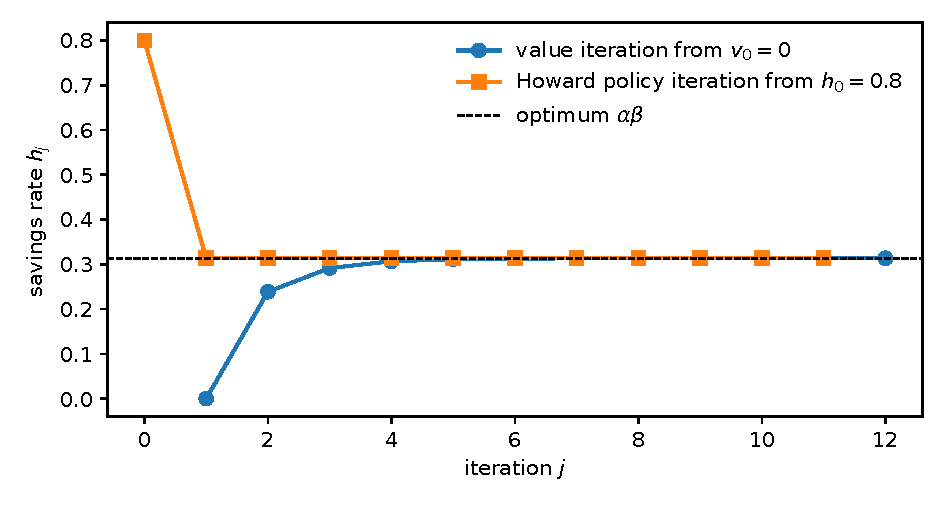
\includegraphics[width=0.9\linewidth]{fig/ls03_policy_iteration.pdf}\\[3pt]
\captionof{figure}{Exercise 3.1. Savings rate $h_j$ by iteration, $\alpha=0.33$, $\beta=0.95$
($\alpha\beta=0.3135$). Howard from $h_0=0.8$ lands on $\alpha\beta$ at $j=1$; value iteration
from $v_0=0$ gives $0,\ 0.2387,\ 0.2917,\ 0.3068,\ 0.3114,\dots$}
\label{fig:pi}
\end{center}

\begin{tcolorbox}[theorybox,title={Why one step is enough}]
The improvement step uses $J_{h_0}$ only through its \emph{derivative} in $k'$ --- the marginal
value of capital. Changing the savings rate rescales consumption in every period and state by
the same factor $(1-h)$, which in logs is an additive constant; and it shifts the mean of
$\ln k$ by a constant. Neither changes how lifetime utility responds to $\ln k$, which is
$\alpha(1+\alpha\beta+(\alpha\beta)^2+\cdots)=\alpha/(1-\alpha\beta)$ for every $h$: a unit of
$\ln k$ today raises $\ln y$ by $\alpha$, and that effect persists at rate $\alpha$ and is
discounted at $\beta$. Since the \emph{wrong} policy already carries the \emph{right} marginal
value of capital, the first improvement is already optimal. Contrast value iteration: there the slope $f_j$ is
built up one term of the geometric series per iteration, and the policy inherits the error.
\end{tcolorbox}

\begin{tcolorbox}[databox]
Notebook \texttt{ls\_ch03.ipynb}, with $A=1$, $\alpha=0.33$, $\beta=0.95$, $\sigma=0.2$ (the
book gives no values).
\begin{itemize}[itemsep=1pt]
\item \eqref{eq:Jh} agrees with the exact mean recursion to $10^{-9}$ and with a 20\,000-path
Monte Carlo within $5$ standard errors, for $h_0\in\{0.1,0.5,0.9\}$.
\item Numerical improvement step (bounded scalar maximisation, $E$ by 20-node Gauss--Hermite):
$h_1\in[0.31349997,\,0.31350002]$ for $h_0\in\{0.05,0.2,0.5,0.8,0.95\}$ and nine states each;
$\alpha\beta=0.3135$. A second step returns the same value.
\item Bellman residual $\max|TJ_{\alpha\beta}-J_{\alpha\beta}|=7\times10^{-15}$ on a grid of
states; for $h_0=0.5$, $TJ_{0.5}-J_{0.5}=0.104>0$ (strict improvement).
\item The value-iteration sequence $h^{VFI}_j$ above matches a numerical Bellman iteration to
$10^{-8}$.
\end{itemize}
\end{tcolorbox}

\begin{tcolorbox}[databox,title={Discretised model --- see the companion notebook}]
Capital on a 250-point geometric grid over $[0.2\bar k,\,4\bar k]$, $\ln\theta$ on 7
Gauss--Hermite nodes (symmetric, so $E\ln\theta'=0$ and the closed form stays the exact
benchmark). Value iteration needs \textbf{450} iterations to reach a sup-norm change below
$10^{-10}$; Howard, started from $h_0=0.25$ and evaluating each policy by solving
$V=R_h+\beta P_hV$, stops after \textbf{5} improvements plus one confirming step. Both give the
identical grid policy, with $k'/y\in[0.3114,\,0.3156]$ on interior states and
$\max|V_{\text{grid}}-V|=8.9\times10^{-5}$.

\smallskip
On the grid, one step is \emph{not} enough: the first improvement leaves
$\max|k'/y-\alpha\beta|=0.0125$, then $0.0058$, $0.0028$, $0.0022$, $0.0021$ (the grid-spacing
floor). Rounding $h_0y$ to the grid breaks the exact form \eqref{eq:Jk}, which the one-step
argument relies on.
\end{tcolorbox}

\begin{center}
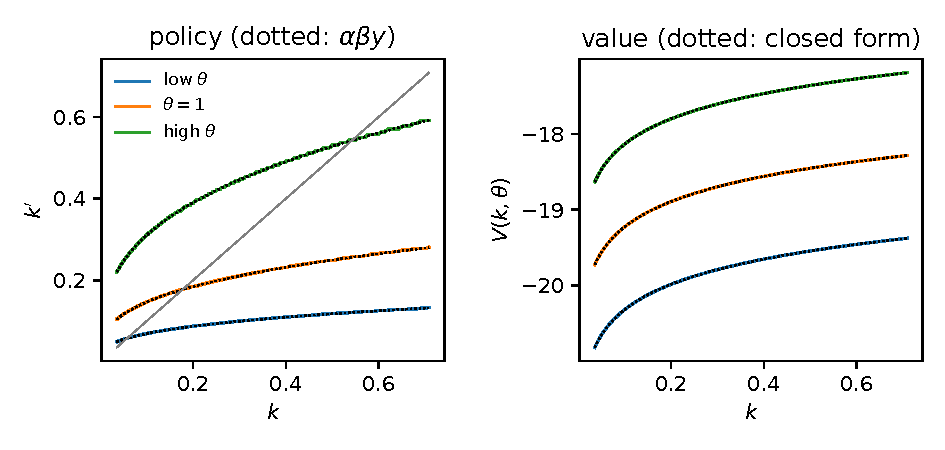
\includegraphics[width=0.95\linewidth]{fig/ls03_discrete.pdf}\\[3pt]
\captionof{figure}{Exercise 3.1, discretised model. Left: grid policy for three shock values
against $\alpha\beta y$ (dotted). Right: grid value function against the closed form
$E+F\ln k+\ln\theta/(1-\alpha\beta)$ (dotted).}
\label{fig:discrete}
\end{center}

\begin{tcolorbox}[trapbox]
\begin{itemize}[itemsep=2pt]
\item \textbf{$E\theta$ is not 1.} With $\ln\theta\sim N(0,\sigma^2)$, $E\theta=e^{\sigma^2/2}$.
What the derivation needs is $E\ln\theta'=0$, and only $\ln\theta$ ever enters because utility
is logarithmic and technology Cobb--Douglas. Using $E\theta=1$ inside a log is Jensen's error.
\item \textbf{Improving over the wrong variable.} The maximisation is over $k'$ with
$J_0$ \emph{held fixed}; do not substitute $k'=h_1y$ into $J_0$'s own $h_0$. The new policy
enters only through the choice of $k'$ today; tomorrow onward the old policy $h_0$ is followed.
\item \textbf{Forgetting the $h$-dependence of the drift.} $\mu_h=\ln A+\alpha\ln h$ depends on
$h$; it matters for the level $a(h)$ and the comparison $J_{\alpha\beta}\ge J_{h}$, even though
it does not affect $h_1$.
\item \textbf{Over-generalising.} One-step convergence is special to the log / Cobb--Douglas /
full-depreciation case, and even there only in the continuous state space: the discretised
version above needs five improvements.
\end{itemize}
\end{tcolorbox}
\end{tcolorbox}

%======================================================================
\section*{Companion code}
\addcontentsline{toc}{section}{Companion code}
%======================================================================

Every numerical result above is reproduced by the notebook \texttt{ls\_ch03.ipynb} in this folder
(executed, outputs saved). Each claim is checked by an independent route with an \texttt{assert}.

\begin{center}
\begin{tabular}{@{}lp{10.2cm}@{}}
\toprule
\textbf{Notebook section} & \textbf{What it does} \\
\midrule
Step 1 & Closed form \eqref{eq:Jh} vs exact mean recursion and Monte Carlo. \\
Step 2 & Numerical improvement step from five values of $h_0$; $h_1=h_2=\alpha\beta$. \\
Step 3 & Bellman residual of $J_{\alpha\beta}$; strict improvement for $h\neq\alpha\beta$. \\
Contrast & Value-iteration savings rates, closed form vs numerical; Figure~\ref{fig:pi}. \\
Discretised & Grid VFI vs grid PFI (identical policies and values), comparison with the
closed form; Figure~\ref{fig:discrete}. \\
\bottomrule
\end{tabular}
\end{center}

Figures are saved to \texttt{fig/ls03\_*.pdf} with TrueType (not Type~3) fonts.

\end{document}
